\chapter*{ INTÉGRATION ET DÉPLOIEMENT}
\addcontentsline{toc}{chapter}{ INTÉGRATION ET DÉPLOIEMENT}

\section{Interface Utilisateur}

\subsection{Interface web avec ADK}

Google ADK révolutionne la création d'interfaces utilisateur pour les systèmes multi-agents en fournissant une interface web moderne et réactive out-of-the-box. Cette interface, basée sur les dernières technologies web, offre une expérience utilisateur fluide et intuitive parfaitement adaptée aux besoins des agriculteurs camerounais.

• Selection de l'agent\\
\begin{figure}[H]
\centering
\framebox[0.9\textwidth]{
\parbox{0.9\textwidth}{
\centering
\textbf{Interface Web Agriculture Cameroun}\\[10pt]

\includegraphics[width=0.9\textwidth]{images/interface_principale.png}\\[5pt]
}
}
\caption{Interface web principale du système}
\end{figure}

• Barre de chat intuitive en bas\\
\begin{figure}[H]
\centering
\framebox[0.9\textwidth]{
\parbox{0.9\textwidth}{
\centering
\textbf{Interface Web Agriculture Cameroun}\\[10pt]
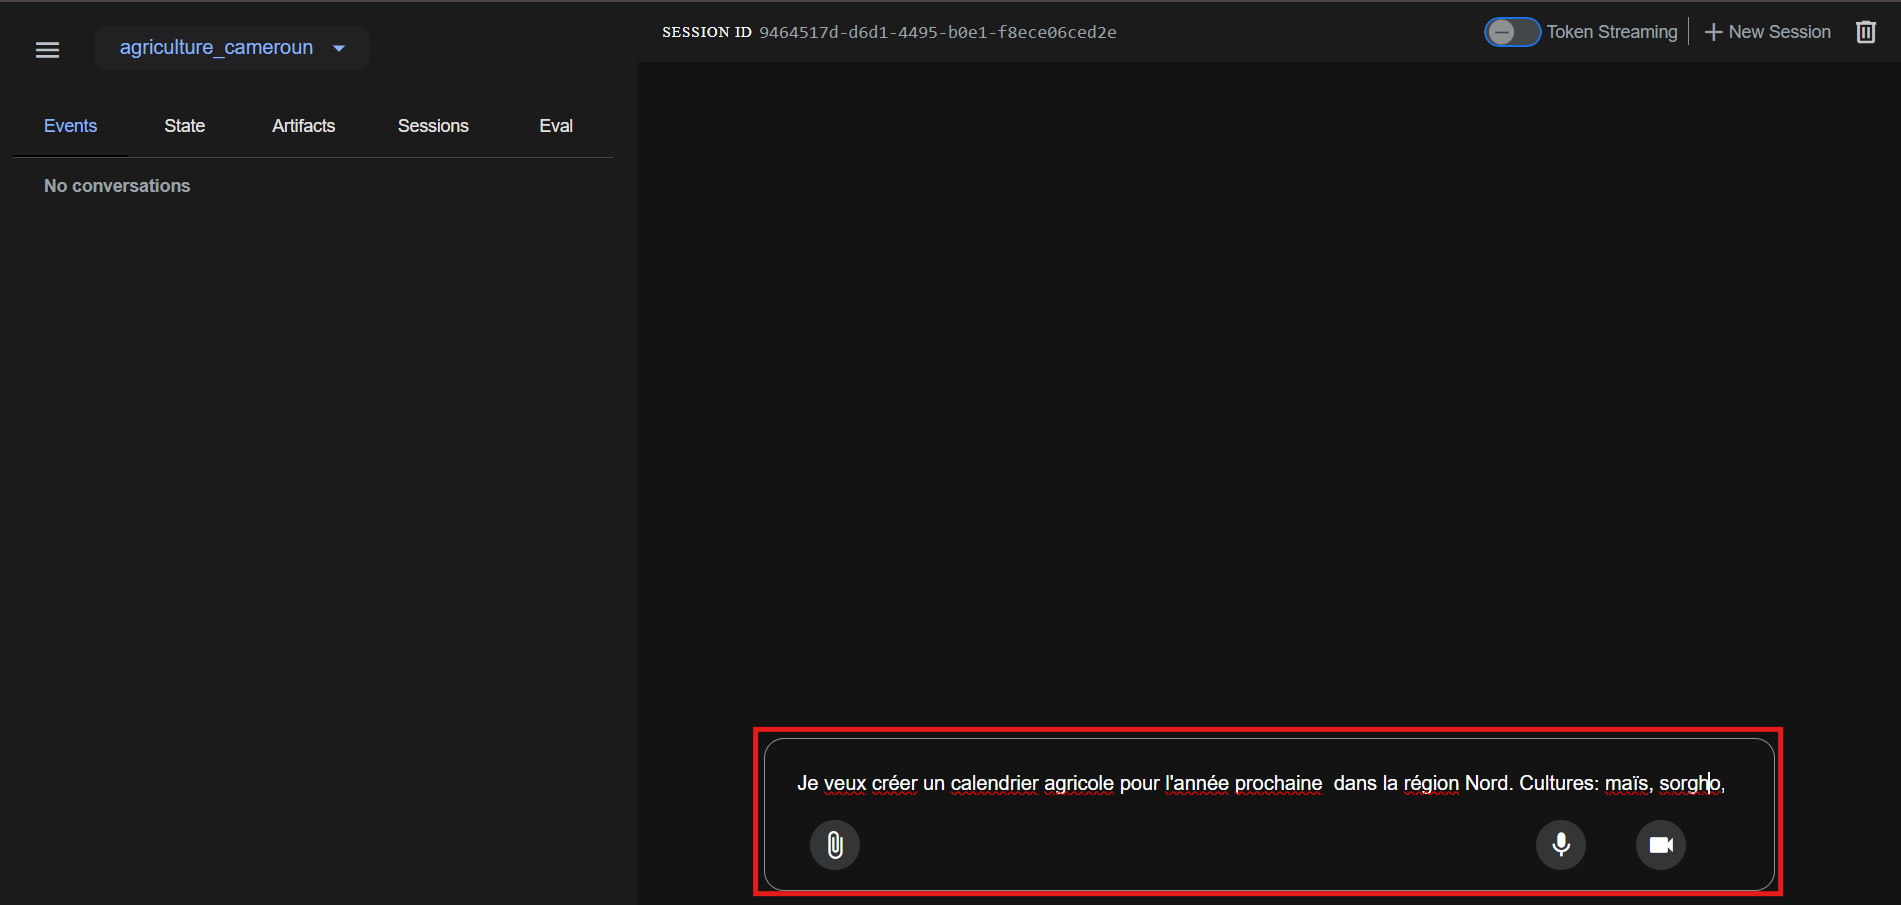
\includegraphics[width=0.9\textwidth]{images/interface_principale_1.png}\\[5pt]
}
}
\caption{Interface web principale du système}
\end{figure}

• Zone de réponse principale au centre\\
\begin{figure}[H]
\centering
\framebox[0.9\textwidth]{
\parbox{0.9\textwidth}{
\centering
\textbf{Interface Web Agriculture Cameroun}\\[10pt]
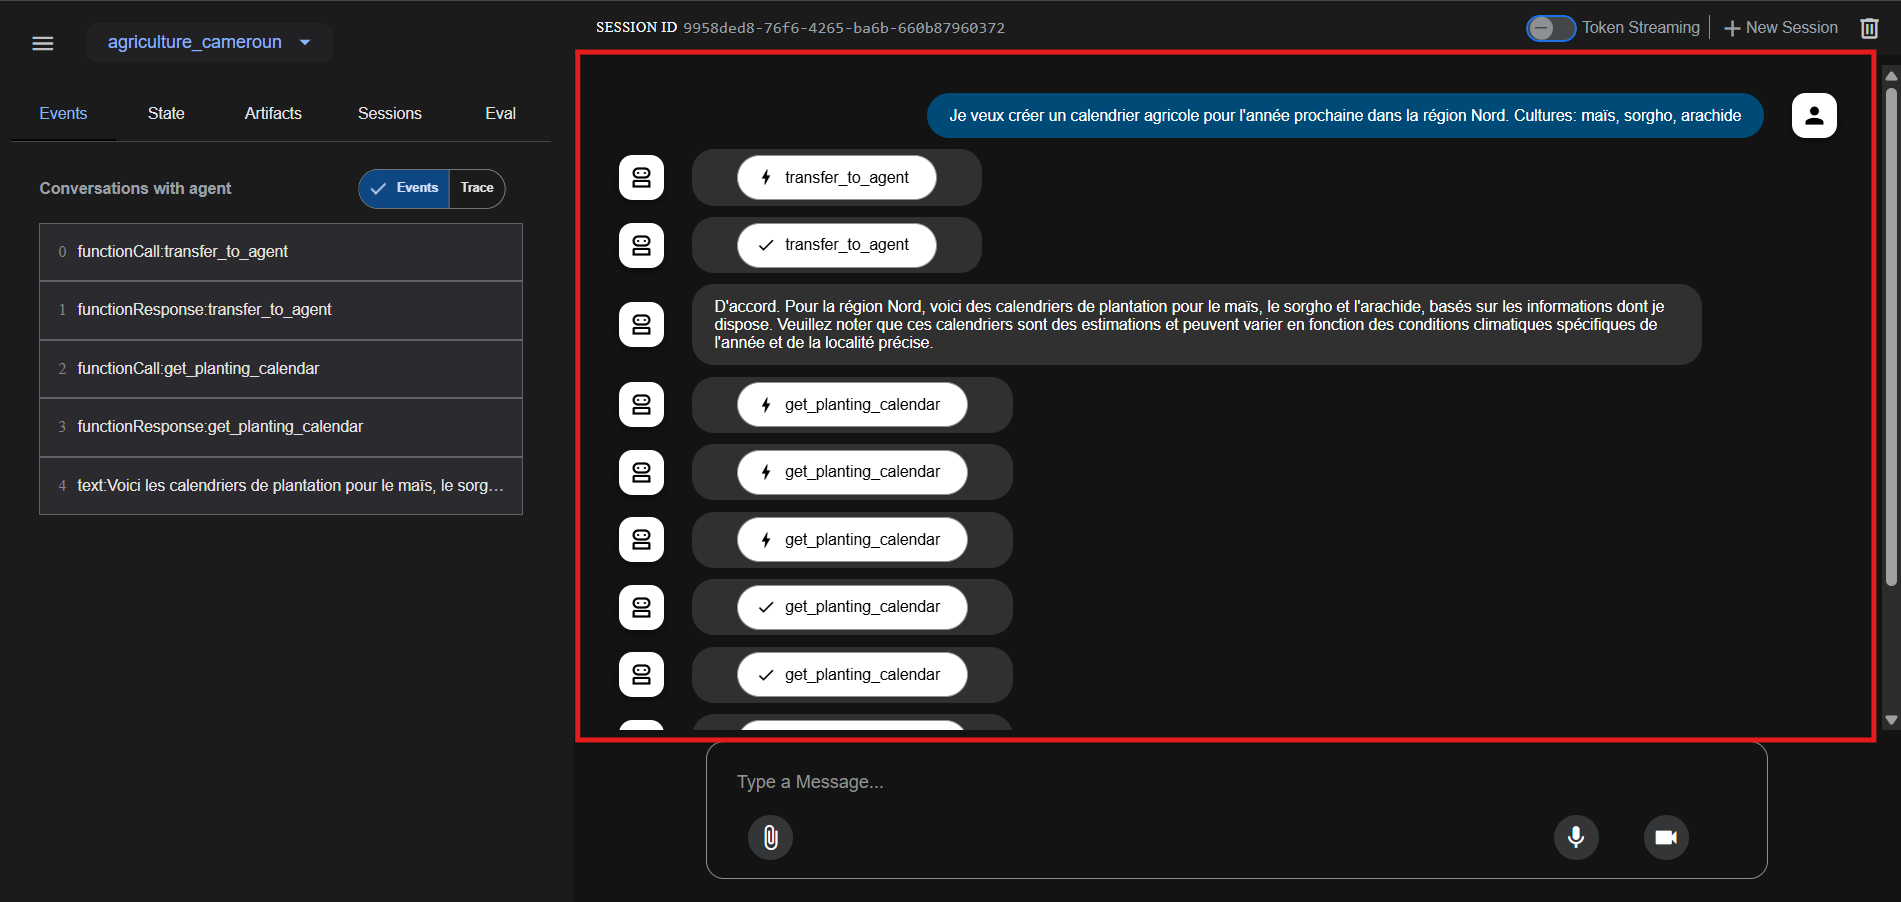
\includegraphics[width=0.9\textwidth]{images/interface_principale_2.png}\\[5pt]
}
}
\caption{Interface web principale du système}
\end{figure}
• Indicateur d'agent actif en temps réel\\[10pt]
\begin{figure}[H]
\centering
\framebox[0.9\textwidth]{
\parbox{0.9\textwidth}{
\centering
\textbf{Interface Web Agriculture Cameroun}\\[10pt]
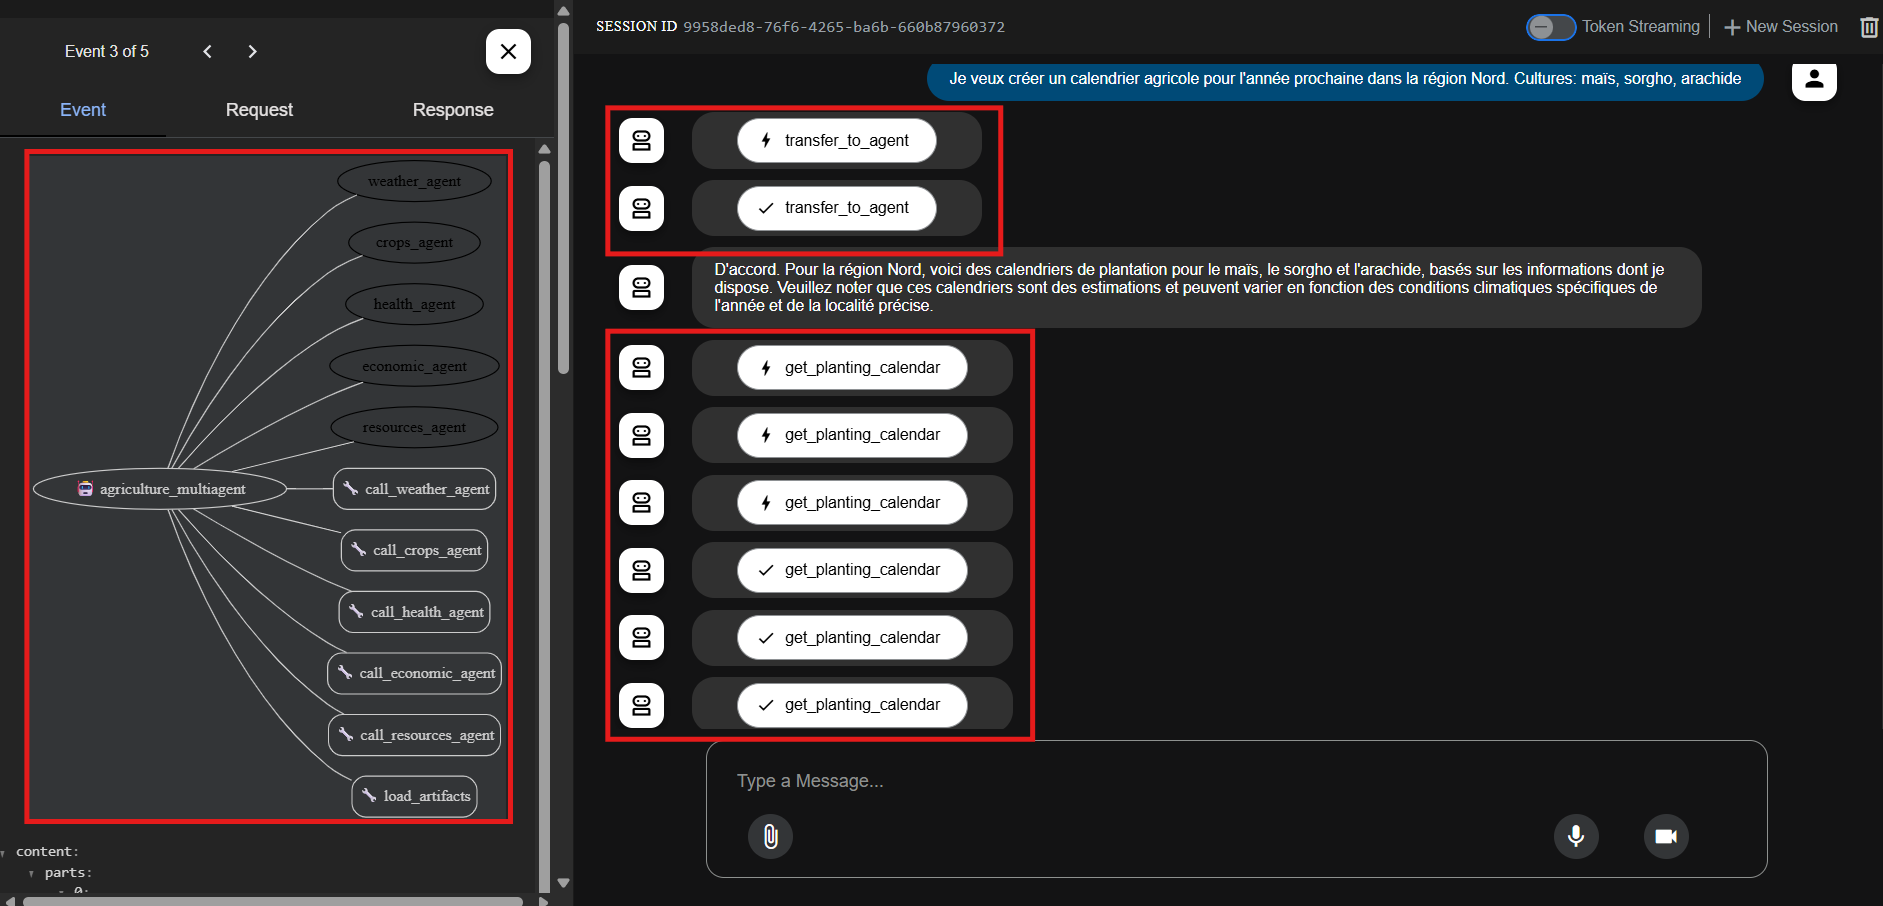
\includegraphics[width=0.9\textwidth]{images/interface_principale_3.png}\\[5pt]
}
}
\caption{Interface web principale du système}
\end{figure}
• URL d'accès : \texttt{http://localhost:8000}\\
• Responsive design adapté mobile/desktop

L'interface web ADK est automatiquement générée lors du lancement du système avec la commande \texttt{poetry run adk web}. Cette approche zero-configuration permet de démarrer immédiatement sans configuration complexe d'interface.

\begin{figure}[H]
\centering
\begin{lstlisting}[language=Python, caption=Configuration de l'interface web ADK]
# Configuration dans agent.py pour personnaliser l'interface

# Configuration des métadonnées d'interface
INTERFACE_CONFIG = {
    "title": "Agriculture Cameroun - Assistant Intelligent",
    "description": "Votre conseiller agricole virtuel disponible 24/7",
    "theme": {
        "primary_color": "#2E7D32",  # Vert agriculture
        "secondary_color": "#FFC107",  # Jaune maïs
        "font_family": "Inter, sans-serif",
        "chat_width": "100%",
        "max_width": "1200px"
    },
    "welcome_message": """
    �� Bienvenue sur Agriculture Cameroun !

    Je suis votre assistant agricole intelligent. Je peux vous aider avec :
    - ��️ Prévisions météo et conseils climatiques
    - �� Recommandations de cultures et calendriers
    - �� Diagnostic de maladies et ravageurs
    - �� Analyse économique et prix du marché
    - �� Gestion optimale des ressources

    Posez-moi vos questions en français ou en anglais !
    """,
    "suggested_queries": [
        "Quand planter le maïs dans la région Centre ?",
        "Mon cacao a des taches brunes, que faire ?",
        "Prix actuel du café arabica au marché",
        "Comment économiser l'eau en saison sèche ?",
        "Prévisions météo pour Douala cette semaine"
    ],
    "features": {
        "voice_input": True,  # Activation entrée vocale
        "file_upload": True,  # Upload photos pour diagnostic
        "export_chat": True,  # Export des conversations
        "offline_mode": False,  # Mode hors ligne (futur)
        "multi_language": ["fr", "en"]  # Langues supportées
    }
}


\end{lstlisting}
\end{figure}

L'interface web intègre des fonctionnalités avancées spécifiquement conçues pour le contexte agricole camerounais. La \textbf{saisie vocale} permet aux agriculteurs ayant une alphabétisation limitée d'interagir naturellement avec le système. L'\textbf{upload d'images} facilite le diagnostic visuel des maladies et ravageurs. Le \textbf{mode sombre automatique} s'adapte aux conditions d'utilisation en extérieur.

\begin{figure}[H]
\centering
\framebox[0.9\textwidth]{
\parbox{0.85\textwidth}{
\centering
\textbf{Fonctionnalités Avancées de l'Interface}\\[10pt]
\textbf{1. Dashboard Agricole Personnalisé}\\
• Météo locale en temps réel\\
• Alertes personnalisées (maladies, météo, marché)\\
• Calendrier cultural interactif\\
• Suivi des activités agricoles\\[5pt]
\textbf{2. Mode Conversation Contextuelle}\\
• Historique persistant par session\\
• Suggestions basées sur le contexte\\
• Reprise de conversation après interruption\\
• Export PDF des recommandations\\[5pt]
\textbf{3. Visualisations Intelligentes}\\
• Graphiques de tendances de prix\\
• Cartes météo interactives\\
• Diagrammes de diagnostic\\
• Tableaux comparatifs de cultures
}
}
\caption{Capacités avancées de l'interface web}
\end{figure}

\subsection{API REST pour intégrations externes}

Au-delà de l'interface web, ADK expose automatiquement une API REST complète permettant l'intégration du système Agriculture Cameroun dans d'autres applications et services.

\begin{figure}[H]
\centering
\begin{lstlisting}[language=Python, caption=Points d'entrée de l'API REST]
# Configuration de l'API REST
# Fichier complet : agriculture/api/rest_api.py

from fastapi import FastAPI, HTTPException, Body
from pydantic import BaseModel, Field
from typing import Optional, List, Dict
import adk

# Modèles de données pour l'API
class QueryRequest(BaseModel):
    """Modèle pour les requêtes utilisateur."""
    query: str = Field(..., description="Question de l'utilisateur")
    session_id: Optional[str] = Field(None, description="ID de session")
    context: Optional[Dict] = Field(None, description="Contexte additionnel")
    language: str = Field("fr", description="Langue de réponse")
    region: Optional[str] = Field(None, description="Région spécifique")

class QueryResponse(BaseModel):
    """Modèle pour les réponses du système."""
    response: str = Field(..., description="Réponse générée")
    agents_consulted: List[str] = Field(..., description="Agents consultés")
    confidence: float = Field(..., description="Score de confiance")
    suggestions: List[str] = Field(..., description="Questions suggérées")
    metadata: Dict = Field(..., description="Métadonnées additionnelles")

# Initialisation de l'API
app = FastAPI(
    title="Agriculture Cameroun API",
    description="API REST pour l'assistant agricole intelligent",
    version="1.0.0",
    docs_url="/api/docs",  # Documentation Swagger
    redoc_url="/api/redoc"  # Documentation ReDoc
)

# Points d'entrée principaux
@app.post("/api/query", response_model=QueryResponse)
async def process_query(request: QueryRequest):
    """
    Traite une requête agricole.

    Exemples:
    - Prévisions météo: "Quelle est la météo à Yaoundé?"
    - Conseils cultures: "Quand planter le maïs?"
    - Diagnostic: "Feuilles jaunes sur tomates"
    """
    try:
        # Traitement de la requête
        result = await agriculture_system.process_query(
            query=request.query,
            session_id=request.session_id,
            context=request.context,
            language=request.language
        )

        return QueryResponse(
            response=result["response"],
            agents_consulted=result["agents_used"],
            confidence=result["confidence"],
            suggestions=result["follow_up_questions"],
            metadata=result["metadata"]
        )
    except Exception as e:
        raise HTTPException(status_code=500, detail=str(e))

@app.get("/api/weather/{region}")
async def get_weather_forecast(
    region: str,
    days: int = 7
):
    """Obtient les prévisions météo pour une région."""
    # Implémentation directe via l'agent météo
    pass

@app.post("/api/diagnose")
async def diagnose_plant_issue(
    crop: str = Body(...),
    symptoms: List[str] = Body(...),
    photos: Optional[List[str]] = Body(None)
):
    """Diagnostique un problème de culture."""
    # Utilisation de l'agent santé des plantes
    pass

@app.get("/api/market/prices")
async def get_market_prices(
    crop: Optional[str] = None,
    region: Optional[str] = None
):
    """Récupère les prix actuels du marché."""
    # Via l'agent économique
    pass

# Endpoints spécialisés pour intégrations
@app.post("/api/bulk/recommendations")
async def get_bulk_recommendations(
    farmers: List[Dict] = Body(...)
):
    """
    Génère des recommandations pour plusieurs agriculteurs.
    Utile pour les coopératives et organisations.
    """
    results = []
    for farmer in farmers:
        recommendation = await generate_personalized_plan(farmer)
        results.append(recommendation)
    return {"recommendations": results}

# Webhooks pour notifications
@app.post("/api/webhooks/weather-alerts")
async def setup_weather_webhook(
    callback_url: str = Body(...),
    regions: List[str] = Body(...),
    alert_types: List[str] = Body(...)
):
    """Configure des alertes météo automatiques."""
    # Configuration du système de notifications
    pass
\end{lstlisting}
\end{figure}

L'API REST suit les standards RESTful modernes avec documentation automatique via Swagger/OpenAPI. Chaque endpoint est optimisé pour des cas d'usage spécifiques, permettant une intégration flexible dans différents contextes.

\begin{figure}[H]
\centering
\framebox[0.9\textwidth]{
\parbox{0.85\textwidth}{
\centering
\textbf{Documentation Interactive de l'API}\\[10pt]
% \includegraphics[width=0.9\textwidth]{[Interface Swagger montrant :]}\\[5pt]
• Liste complète des endpoints\\
• Modèles de données avec exemples\\
• Interface de test "Try it out"\\
• Authentification via API key\\
• Codes de réponse détaillés\\[10pt]
Accès : \texttt{http://localhost:8000/api/docs}\\[5pt]
\textbf{Exemples de requêtes cURL :}\\[5pt]
\texttt{curl -X POST http://localhost:8000/api/query}\\
\texttt{-H "Content-Type: application/json"}\\
\texttt{-d '\{"query": "Météo Douala demain"\}'}
}
}
\caption{Interface de documentation Swagger de l'API}
\end{figure}

\subsection{Exemples d'utilisation}

Pour illustrer concrètement l'utilisation du système, examinons plusieurs scénarios réels d'interaction avec l'interface.

\begin{figure}[H]
\centering
\framebox[0.9\textwidth]{
\parbox{0.85\textwidth}{
\centering
\textbf{Scénario 1 : Planification de Culture}\\[10pt]
% \includegraphics[width=0.9\textwidth]{[Capture montrant :]}\\[5pt]
\textbf{Utilisateur :} "Je veux commencer la culture du cacao sur 2 hectares à Bafia"\\[5pt]
\textbf{Système :}
• Vérifie conditions climatiques de Bafia (Centre)\\
• Analyse aptitude des sols pour le cacao\\
• Propose calendrier cultural détaillé\\
• Estime investissement initial\\
• Suggère variétés adaptées\\[5pt]
\textit{Interface affiche carte interactive, calendrier et tableau financier}
}
}
\caption{Exemple de planification de nouvelle culture}
\end{figure}

\begin{figure}[H]
\centering
\begin{lstlisting}[language=JavaScript, caption=Intégration JavaScript de l'API]
// Exemple d'intégration dans une application mobile

class AgricultureCamerounClient {
    constructor(apiKey) {
        this.baseUrl = 'https://api.agriculture-cameroun.cm';
        this.apiKey = apiKey;
        this.sessionId = this.generateSessionId();
    }

    async askQuestion(query, context = {}) {
        const response = await fetch(`${this.baseUrl}/api/query`, {
            method: 'POST',
            headers: {
                'Content-Type': 'application/json',
                'X-API-Key': this.apiKey
            },
            body: JSON.stringify({
                query: query,
                session_id: this.sessionId,
                context: context,
                language: navigator.language.startsWith('fr') ? 'fr' : 'en'
            })
        });

        return await response.json();
    }

    async uploadDiseasePhoto(photo, crop, description) {
        // Conversion photo en base64
        const base64Photo = await this.convertToBase64(photo);

        const response = await fetch(`${this.baseUrl}/api/diagnose`, {
            method: 'POST',
            headers: {
                'Content-Type': 'application/json',
                'X-API-Key': this.apiKey
            },
            body: JSON.stringify({
                crop: crop,
                symptoms: this.extractSymptoms(description),
                photos: [base64Photo]
            })
        });

        const diagnosis = await response.json();
        return this.formatDiagnosisForDisplay(diagnosis);
    }

    // Utilisation avec notifications push
    async subscribeToAlerts(region, alertTypes) {
        const subscription = await this.registerPushNotifications();

        await fetch(`${this.baseUrl}/api/webhooks/alerts`, {
            method: 'POST',
            headers: {
                'Content-Type': 'application/json',
                'X-API-Key': this.apiKey
            },
            body: JSON.stringify({
                callback_url: subscription.endpoint,
                regions: [region],
                alert_types: alertTypes,
                user_preferences: {
                    quiet_hours: "22:00-06:00",
                    language: "fr",
                    urgency_threshold: "medium"
                }
            })
        });
    }
}

// Exemple d'utilisation dans une app React Native
const agriClient = new AgricultureCamerounClient('your-api-key');

// Conversation simple
const response = await agriClient.askQuestion(
    "Mes tomates ont des feuilles qui jaunissent par le bas"
);
console.log(response.response); // Diagnostic et recommandations

// Upload photo pour diagnostic
const diagnosis = await agriClient.uploadDiseasePhoto(
    photoFile,
    'tomate',
    'Jaunissement progressif des feuilles basales'
);

// Souscription aux alertes
await agriClient.subscribeToAlerts('Ouest', [
    'extreme_weather',
    'disease_outbreak',
    'market_opportunity'
]);
\end{lstlisting}
\end{figure}

\begin{figure}[H]
\centering
\framebox[0.9\textwidth]{
\parbox{0.85\textwidth}{
\centering
\textbf{Scénario 2 : Diagnostic Visuel par Photo}\\[10pt]
% \includegraphics[width=0.9\textwidth]{[Interface montrant :]}\\[5pt]
1. Bouton "�� Prendre une photo" prominent\\
2. Zone de preview de l'image uploadée\\
3. Analyse en temps réel avec indicateur de progression\\
4. Résultats structurés :\\
   • Maladie identifiée avec \% confiance\\
   • Zones affectées surlignées sur la photo\\
   • Plan de traitement étape par étape\\
   • Produits recommandés avec dosages\\[5pt]
\textit{Particulièrement utile pour diagnostics complexes}
}
}
\caption{Interface de diagnostic visuel des maladies}
\end{figure}

\section{Tests et Validation}

\subsection{Tests unitaires des agents}

La stratégie de test du système Agriculture Cameroun assure la fiabilité et la précision des conseils fournis aux agriculteurs. Chaque agent dispose de sa propre suite de tests couvrant ses fonctionnalités spécifiques.

\begin{figure}[H]
\centering
\begin{lstlisting}[language=Python, caption=Framework de tests unitaires pour agents ADK]
# Structure de tests dans tests/unit/test_agents.py
import pytest
from unittest.mock import Mock, patch
import adk
from agriculture.sub_agents.weather.agent import weather_agent
from agriculture.sub_agents.crops.agent import crops_agent

class TestWeatherAgent:
    """Tests unitaires pour l'agent météorologique."""

    @pytest.fixture
    def mock_weather_api(self):
        """Mock des appels API météo externes."""
        with patch('requests.get') as mock_get:
            mock_get.return_value.json.return_value = {
                "temperature": 28,
                "humidity": 75,
                "precipitation": 0,
                "forecast": "sunny"
            }
            yield mock_get

    def test_weather_forecast_accuracy(self, mock_weather_api):
        """Teste la précision des prévisions météo."""
        # Configuration du test
        query = "Météo pour Yaoundé demain"
        expected_keywords = ["température", "humidité", "ensoleillé"]

        # Exécution
        response = weather_agent.run(query)

        # Vérifications
        assert response.success
        assert all(keyword in response.content.lower()
                  for keyword in expected_keywords)
        assert "28" in response.content  # Température
        assert mock_weather_api.called

    def test_agricultural_alerts(self):
        """Teste la génération d'alertes agricoles."""
        # Simulation conditions extrêmes
        extreme_conditions = {
            "temperature": 40,
            "humidity": 30,
            "wind_speed": 45
        }

        with patch('agriculture.tools.get_weather_data',
                  return_value=extreme_conditions):
            response = weather_agent.run(
                "Conditions pour pulvérisation aujourd'hui?"
            )

            # Doit déconseiller la pulvérisation
            assert "déconseillé" in response.content.lower()
            assert "vent" in response.content.lower()
            assert "température" in response.content.lower()

    @pytest.mark.parametrize("region,expected_pattern", [
        ("Nord", "saison sèche|harmattan"),
        ("Littoral", "pluie|humidité élevée"),
        ("Ouest", "altitude|fraîcheur"),
    ])
    def test_regional_specificity(self, region, expected_pattern):
        """Teste l'adaptation aux spécificités régionales."""
        import re

        query = f"Climat typique de la région {region}"
        response = weather_agent.run(query)

        assert re.search(expected_pattern, response.content, re.IGNORECASE)

class TestCropsAgent:
    """Tests unitaires pour l'agent cultures."""

    def test_crop_calendar_generation(self):
        """Teste la génération de calendriers culturaux."""
        query = "Calendrier cultural du maïs pour Garoua"
        response = crops_agent.run(query)

        # Vérification des éléments essentiels
        calendar_elements = [
            "préparation du sol",
            "semis",
            "sarclage",
            "fertilisation",
            "récolte"
        ]

        assert all(element in response.content.lower()
                  for element in calendar_elements)

        # Vérification des périodes spécifiques à Garoua
        assert any(month in response.content
                  for month in ["mai", "juin"])  # Période de semis

    def test_crop_recommendations_constraints(self):
        """Teste les recommandations avec contraintes."""
        query = """
        Quelle culture pour :
        - Sol argileux pH 5.5
        - Budget limité (100,000 FCFA/ha)
        - Main d'œuvre familiale seulement
        - Région Centre
        """

        response = crops_agent.run(query)

        # Doit recommander cultures adaptées
        assert "manioc" in response.content.lower() or \
               "plantain" in response.content.lower()

        # Doit mentionner l'adaptation au sol acide
        assert "pH" in response.content or "acide" in response.content

        # Doit considérer le budget
        assert "budget" in response.content.lower()

# Tests d'intégration des outils
class TestAgentTools:
    """Tests des outils utilisés par les agents."""

    def test_soil_analysis_tool(self):
        """Teste l'outil d'analyse du sol."""
        from agriculture.sub_agents.resources.tools import analyze_soil_data

        result = analyze_soil_data(
            ph=6.5,
            organic_matter_percent=2.5,
            nitrogen_ppm=15,
            phosphorus_ppm=25,
            potassium_ppm=180,
            texture="loamy",
            crop_planned="cacao"
        )

        assert "soil_health_score" in result
        assert 60 <= result["soil_health_score"] <= 80
        assert "recommendations" in result
        assert len(result["recommendations"]) > 0

    def test_disease_diagnostic_tool(self):
        """Teste l'outil de diagnostic des maladies."""
        from agriculture.sub_agents.health.tools import diagnose_plant_disease

        diagnosis = diagnose_plant_disease(
            crop="tomate",
            symptoms=["feuilles jaunes", "taches brunes", "flétrissement"],
            affected_parts=["feuilles", "tige"],
            development_stage="floraison"
        )

        assert "possible_diseases" in diagnosis
        assert len(diagnosis["possible_diseases"]) > 0
        assert diagnosis["possible_diseases"][0]["probability"] > 50
        assert "treatment_plan" in diagnosis

# Tests de performance
class TestPerformance:
    """Tests de performance du système."""

    @pytest.mark.benchmark
    def test_response_time(self, benchmark):
        """Teste le temps de réponse des agents."""
        query = "Quand planter le maïs à Yaoundé?"

        # Benchmark de la performance
        result = benchmark(weather_agent.run, query)

        assert result.success
        # Temps de réponse acceptable < 2 secondes
        assert benchmark.stats['mean'] < 2.0

    def test_concurrent_requests(self):
        """Teste la gestion de requêtes concurrentes."""
        import asyncio
        from concurrent.futures import ThreadPoolExecutor

        queries = [
            "Météo Douala",
            "Prix du cacao",
            "Maladies du maïs",
            "Calendrier cultural café",
            "Analyse sol argileux"
        ]

        with ThreadPoolExecutor(max_workers=5) as executor:
            futures = [executor.submit(process_query, q) for q in queries]
            results = [f.result() for f in futures]

        assert all(r is not None for r in results)
        assert len(results) == len(queries)
\end{lstlisting}
\end{figure}

Les tests unitaires couvrent non seulement la fonctionnalité correcte mais aussi la \textbf{pertinence agricole} des réponses. Des tests spécifiques vérifient que les recommandations sont adaptées au contexte camerounais et suivent les bonnes pratiques agricoles locales.

\subsection{Tests d'intégration}

Les tests d'intégration vérifient que les différents composants du système fonctionnent harmonieusement ensemble, particulièrement important pour un système multi-agents où la coordination est cruciale.

\begin{figure}[H]
\centering
\begin{lstlisting}[language=Python, caption=Suite de tests d'intégration]
# Tests d'intégration dans tests/integration/test_system.py
import pytest
from agriculture import main_agent
import time

class TestMultiAgentIntegration:
    """Tests d'intégration du système complet."""

    @pytest.fixture(scope="class")
    def system_instance(self):
        """Instance du système pour les tests."""
        # Configuration de test
        test_config = {
            "default_region": "Centre",
            "default_language": "fr",
            "test_mode": True
        }
        return main_agent.MainCoordinatorAgent(test_config)

    def test_complex_query_routing(self, system_instance):
        """Teste le routage de requêtes complexes."""
        # Requête nécessitant plusieurs agents
        complex_query = """
        Je veux planter du maïs le mois prochain à Bafoussam.
        Quelle est la météo prévue et quel budget prévoir?
        Y a-t-il des risques de maladies en cette période?
        """

        response = system_instance.process_query(complex_query)

        # Vérifications multi-agents
        assert "météo" in response.lower() or "pluie" in response.lower()
        assert "budget" in response.lower() or "coût" in response.lower()
        assert "maladie" in response.lower() or "risque" in response.lower()

        # Vérifier cohérence temporelle
        assert "mois prochain" in response.lower() or \
               any(month in response.lower()
                   for month in ["avril", "mai", "juin"])

    def test_context_preservation(self, system_instance):
        """Teste la préservation du contexte entre requêtes."""
        session_id = "test_session_123"

        # Première requête
        response1 = system_instance.process_query(
            "Je cultive du cacao dans l'Ouest",
            session_id=session_id
        )

        # Deuxième requête utilisant contexte implicite
        response2 = system_instance.process_query(
            "Quelles sont les maladies courantes?",
            session_id=session_id
        )

        # Doit mentionner maladies du cacao, pas général
        assert "cacao" in response2.lower()
        assert any(disease in response2.lower()
                  for disease in ["pourriture", "swollen shoot"])

    def test_error_recovery(self, system_instance):
        """Teste la récupération d'erreurs."""
        # Simulation d'erreur d'un sous-agent
        with patch('agriculture.sub_agents.weather.agent.run',
                  side_effect=Exception("API météo indisponible")):

            response = system_instance.process_query(
                "Météo et conseils pour planter demain"
            )

            # Doit quand même fournir conseils cultures
            assert "planter" in response.lower()
            # Doit mentionner problème météo
            assert "météo" in response.lower()
            assert "non disponible" in response.lower() or \
                   "problème" in response.lower()

class TestEndToEndScenarios:
    """Tests de scénarios complets bout-en-bout."""

    def test_new_farmer_onboarding(self, system_instance):
        """Teste le parcours d'un nouvel agriculteur."""
        session_id = "new_farmer_001"

        # Étape 1: Présentation
        intro = system_instance.process_query(
            "Bonjour, je suis nouveau dans l'agriculture",
            session_id=session_id
        )
        assert "bienvenue" in intro.lower()
        assert any(word in intro.lower()
                  for word in ["aide", "assister", "conseiller"])

        # Étape 2: Contexte
        context_response = system_instance.process_query(
            "J'ai 2 hectares à Dschang, sol volcanique",
            session_id=session_id,
            user_context={"region": "Ouest", "land_size": 2}
        )
        assert "volcanique" in context_response.lower()
        assert "Dschang" in context_response or "Ouest" in context_response

        # Étape 3: Recommandation culturale
        crop_advice = system_instance.process_query(
            "Quelle culture me conseillez-vous?",
            session_id=session_id
        )
        # Doit recommander cultures adaptées à l'Ouest
        assert any(crop in crop_advice.lower()
                  for crop in ["café", "pomme de terre", "maraîcher"])

    def test_seasonal_advisory_flow(self):
        """Teste le flux de conseil saisonnier."""
        # Obtenir saison actuelle
        current_month = time.strftime("%B")
        current_season = get_current_season()

        # Requête contextuelle à la saison
        seasonal_query = f"Que faire ce mois de {current_month}?"
        response = system_instance.process_query(seasonal_query)

        # Doit mentionner activités saisonnières
        if current_season == "planting":
            assert any(word in response.lower()
                      for word in ["semis", "planter", "préparer"])
        elif current_season == "growing":
            assert any(word in response.lower()
                      for word in ["entretien", "sarclage", "fertilisation"])
        elif current_season == "harvest":
            assert any(word in response.lower()
                      for word in ["récolte", "stockage", "vente"])

# Tests de validation des données
class TestDataValidation:
    """Valide l'exactitude des données agricoles."""

    def test_crop_calendar_accuracy(self):
        """Vérifie l'exactitude des calendriers culturaux."""
        from agriculture.utils.data import CROP_CALENDARS

        # Vérifier cohérence des données
        for crop, calendar in CROP_CALENDARS.items():
            for region, timing in calendar.items():
                # Les périodes doivent être valides
                assert 1 <= timing["planting_month"] <= 12
                assert timing["growth_duration"] > 0
                assert timing["growth_duration"] < 365

                # Logique agricole
                if crop == "maïs":
                    # Le maïs a un cycle de 90-120 jours
                    assert 90 <= timing["growth_duration"] <= 120

    def test_price_data_reasonableness(self):
        """Vérifie la cohérence des données de prix."""
        from agriculture.utils.data import MARKET_PRICES

        for crop, prices in MARKET_PRICES.items():
            # Les prix doivent être positifs et raisonnables
            assert prices["min"] > 0
            assert prices["max"] > prices["min"]
            assert prices["average"] > prices["min"]
            assert prices["average"] < prices["max"]

            # Vérification de cohérence par culture
            if crop == "cacao":
                # Prix du cacao en FCFA/kg
                assert 800 <= prices["average"] <= 2000
\end{lstlisting}
\end{figure}

\subsection{Scénarios de test complets}

Les scénarios de test complets simulent des cas d'usage réels pour valider que le système répond correctement aux besoins des agriculteurs camerounais.

\begin{figure}[H]
\centering
\framebox[0.9\textwidth]{
\parbox{0.85\textwidth}{
\centering
\textbf{Scénarios de Test Automatisés}\\[10pt]
�� Localisation : \texttt{tests/scenarios/}\\[10pt]
\textbf{Scénarios critiques testés :}\\[5pt]
1. \textbf{Urgence Phytosanitaire}\\
   • Détection rapide invasion ravageurs\\
   • Mobilisation multi-agents\\
   • Plan d'action immédiat\\[5pt]
2. \textbf{Planification Saisonnière}\\
   • Analyse conditions initiales\\
   • Recommandations coordonnées\\
   • Suivi sur cycle complet\\[5pt]
3. \textbf{Optimisation Économique}\\
   • Analyse rentabilité multi-cultures\\
   • Adaptation aux prix marché\\
   • Stratégies de diversification\\[5pt]
4. \textbf{Adaptation Climatique}\\
   • Réponse aux alertes météo\\
   • Ajustement des pratiques\\
   • Résilience long terme
}
}
\caption{Scénarios de test end-to-end}
\end{figure}

\section{Déploiement}

\subsection{Déploiement local}

Le déploiement local du système Agriculture Cameroun est conçu pour être simple et rapide, permettant aux développeurs et testeurs de démarrer immédiatement.

\begin{figure}[H]
\centering
\begin{lstlisting}[language=bash, caption=Script de déploiement local automatisé]
#!/bin/bash
# Script de déploiement local : scripts/deploy_local.sh

echo "�� Déploiement local d'Agriculture Cameroun"
echo "=========================================="

# Vérification des prérequis
check_requirements() {
    echo "Vérification des prérequis..."

    # Python 3.12+
    if ! python3 --version | grep -E "3\.(1[2-9]|[2-9][0-9])" > /dev/null; then
        echo "❌ Python 3.12+ requis"
        exit 1
    fi

    # Poetry
    if ! command -v poetry &> /dev/null; then
        echo "�� Installation de Poetry..."
        curl -sSL https://install.python-poetry.org | python3 -
        export PATH="$HOME/.local/bin:$PATH"
    fi

    # Git
    if ! command -v git &> /dev/null; then
        echo "❌ Git requis pour le déploiement"
        exit 1
    fi

    echo "✅ Tous les prérequis sont satisfaits"
}

# Installation du projet
install_project() {
    echo -e "\n�� Installation du projet..."

    # Clone ou mise à jour
    if [ -d "agriculture-cameroun" ]; then
        cd agriculture-cameroun
        git pull origin main
    else
        git clone https://github.com/Nameless0l/agriculture-cameroun.git
        cd agriculture-cameroun
    fi

    # Installation des dépendances
    echo "�� Installation des dépendances Python..."
    poetry install --no-interaction --verbose

    # Configuration de l'environnement
    if [ ! -f ".env" ]; then
        echo -e "\n⚙️ Configuration de l'environnement..."
        cp .env.example .env

        # Demander la clé API Gemini
        read -p "Entrez votre clé API Gemini: " gemini_key
        sed -i "s/your_gemini_api_key_here/$gemini_key/" .env

        # Configuration régionale
        echo "Sélectionnez votre région par défaut:"
        select region in "Centre" "Littoral" "Ouest" "Nord" "Sud" "Est"; do
            sed -i "s/DEFAULT_REGION=.*/DEFAULT_REGION=$region/" .env
            break
        done
    fi
}

# Lancement du système
start_system() {
    echo -e "\n�� Lancement du système..."

    # Activation de l'environnement Poetry
    poetry shell

    # Vérification de la configuration
    python scripts/check_config.py
    if [ $? -ne 0 ]; then
        echo "❌ Erreur de configuration"
        exit 1
    fi

    # Lancement avec ADK
    echo -e "\n✨ Démarrage d'Agriculture Cameroun..."
    echo "�� Interface web : http://localhost:8000"
    echo "�� Documentation API : http://localhost:8000/api/docs"
    echo -e "\nAppuyez sur Ctrl+C pour arrêter le serveur\n"

    # Lancement avec options de développement
    ADK_DEV_MODE=true ADK_LOG_LEVEL=INFO adk web --port 8000 --reload
}

# Menu principal
main_menu() {
    clear
    echo "�� Agriculture Cameroun - Déploiement Local"
    echo "==========================================="
    echo "1. Installation complète (première fois)"
    echo "2. Mise à jour et lancement"
    echo "3. Lancement seulement"
    echo "4. Tests du système"
    echo "5. Quitter"

    read -p "Choisissez une option (1-5): " choice

    case $choice in
        1)
            check_requirements
            install_project
            start_system
            ;;
        2)
            cd agriculture-cameroun
            git pull origin main
            poetry install
            start_system
            ;;
        3)
            cd agriculture-cameroun
            start_system
            ;;
        4)
            cd agriculture-cameroun
            poetry run pytest tests/ -v
            ;;
        5)
            echo "Au revoir ! ��"
            exit 0
            ;;
        *)
            echo "Option invalide"
            sleep 2
            main_menu
            ;;
    esac
}

# Point d'entrée
main_menu
\end{lstlisting}
\end{figure}

Le déploiement local inclut des \textbf{outils de développement avancés} comme le rechargement automatique du code, les logs détaillés et l'accès aux outils de débogage ADK. Le mode développement active également des endpoints supplémentaires pour tester individuellement chaque agent.

\subsection{Containerisation avec Docker}

La containerisation Docker assure une portabilité parfaite et simplifie grandement le déploiement en production.

\begin{figure}[H]
\centering
\begin{lstlisting}[language=Dockerfile, caption=Docker optimisé pour Agriculture Cameroun]
# Dockerfile multi-stage pour optimisation
FROM python:3.12-slim as builder

# Variables d'environnement pour optimisation
ENV PYTHONUNBUFFERED=1 \
    PYTHONDONTWRITEBYTECODE=1 \
    POETRY_VERSION=1.7.0 \
    POETRY_HOME="/opt/poetry" \
    POETRY_VIRTUALENVS_IN_PROJECT=true \
    POETRY_NO_INTERACTION=1

# Installation de Poetry
RUN apt-get update && apt-get install -y \
    curl \
    build-essential \
    && curl -sSL https://install.python-poetry.org | python3 - \
    && apt-get clean \
    && rm -rf /var/lib/apt/lists/*

ENV PATH="$POETRY_HOME/bin:$PATH"

# Copie des fichiers de dépendances
WORKDIR /app
COPY pyproject.toml poetry.lock ./

# Installation des dépendances
RUN poetry install --no-root --no-dev

# Stage de production
FROM python:3.12-slim

ENV PYTHONUNBUFFERED=1 \
    PYTHONDONTWRITEBYTECODE=1

# Création utilisateur non-root
RUN useradd -m -u 1000 agriuser && \
    mkdir -p /app && \
    chown -R agriuser:agriuser /app

WORKDIR /app

# Copie des dépendances depuis builder
COPY --from=builder /app/.venv /app/.venv
ENV PATH="/app/.venv/bin:$PATH"

# Copie du code application
COPY --chown=agriuser:agriuser . .

# Changement vers utilisateur non-root
USER agriuser

# Healthcheck
HEALTHCHECK --interval=30s --timeout=10s --start-period=5s --retries=3 \
    CMD curl -f http://localhost:8000/health || exit 1

# Port d'exposition
EXPOSE 8000

# Commande de démarrage
CMD ["adk", "web", "--host", "0.0.0.0", "--port", "8000"]
\end{lstlisting}
\end{figure}

\begin{figure}[H]
\centering
\begin{lstlisting}[language=yaml, caption=Docker Compose pour environnement complet]
# docker-compose.yml
version: '3.8'

services:
  # Service principal Agriculture Cameroun
  agriculture-api:
    build:
      context: .
      dockerfile: Dockerfile
    image: agriculture-cameroun:latest
    container_name: agriculture_cameroun_api
    ports:
      - "8000:8000"
    environment:
      - GEMINI_API_KEY=${GEMINI_API_KEY}
      - DEFAULT_REGION=${DEFAULT_REGION:-Centre}
      - DEFAULT_LANGUAGE=${DEFAULT_LANGUAGE:-fr}
      - LOG_LEVEL=${LOG_LEVEL:-INFO}
      - REDIS_URL=redis://redis:6379/0
    volumes:
      - ./data:/app/data
      - ./logs:/app/logs
    depends_on:
      - redis
    restart: unless-stopped
    networks:
      - agriculture-network

  # Cache Redis pour performances
  redis:
    image: redis:7-alpine
    container_name: agriculture_redis
    ports:
      - "6379:6379"
    volumes:
      - redis-data:/data
    command: redis-server --appendonly yes
    restart: unless-stopped
    networks:
      - agriculture-network

  # Monitoring avec Prometheus
  prometheus:
    image: prom/prometheus:latest
    container_name: agriculture_prometheus
    ports:
      - "9090:9090"
    volumes:
      - ./monitoring/prometheus.yml:/etc/prometheus/prometheus.yml
      - prometheus-data:/prometheus
    command:
      - '--config.file=/etc/prometheus/prometheus.yml'
      - '--storage.tsdb.path=/prometheus'
    restart: unless-stopped
    networks:
      - agriculture-network

  # Dashboard Grafana
  grafana:
    image: grafana/grafana:latest
    container_name: agriculture_grafana
    ports:
      - "3000:3000"
    environment:
      - GF_SECURITY_ADMIN_PASSWORD=${GRAFANA_PASSWORD:-admin}
    volumes:
      - grafana-data:/var/lib/grafana
      - ./monitoring/grafana/dashboards:/etc/grafana/provisioning/dashboards
    depends_on:
      - prometheus
    restart: unless-stopped
    networks:
      - agriculture-network

  # Nginx reverse proxy
  nginx:
    image: nginx:alpine
    container_name: agriculture_nginx
    ports:
      - "80:80"
      - "443:443"
    volumes:
      - ./nginx/nginx.conf:/etc/nginx/nginx.conf
      - ./nginx/ssl:/etc/nginx/ssl
    depends_on:
      - agriculture-api
    restart: unless-stopped
    networks:
      - agriculture-network

volumes:
  redis-data:
  prometheus-data:
  grafana-data:

networks:
  agriculture-network:
    driver: bridge
\end{lstlisting}
\end{figure}

La configuration Docker Compose fournit un environnement de production complet avec cache Redis pour les performances, monitoring Prometheus/Grafana pour l'observabilité, et Nginx pour la terminaison SSL et le load balancing.

\subsection{Déploiement en production}

Le déploiement en production nécessite des considérations supplémentaires pour assurer la fiabilité, la sécurité et la scalabilité du système.

\begin{figure}[H]
\centering
\framebox[0.9\textwidth]{
\parbox{0.85\textwidth}{
\centering
\textbf{Architecture de Production}\\[10pt]
% \includegraphics[width=0.9\textwidth]{[Diagramme montrant :]}\\[5pt]
• Load Balancer (Nginx/HAProxy)\\
• Cluster ADK multi-instances\\
• Cache distribué Redis\\
• Base de données PostgreSQL\\
• Storage object pour médias\\
• CDN pour assets statiques\\
• Monitoring stack complet\\[10pt]
\textbf{Plateformes Cloud Supportées :}\\
✓ Google Cloud Platform (recommandé)\\
✓ AWS (EC2, ECS, Lambda)\\
✓ Azure (Container Instances)\\
✓ DigitalOcean (Apps Platform)\\
✓ Serveurs dédiés on-premise
}
}
\caption{Architecture de déploiement production}
\end{figure}

\begin{figure}[H]
\centering
\begin{lstlisting}[language=bash, caption=Script de déploiement production (GCP)]
#!/bin/bash
# deploy_production_gcp.sh - Déploiement sur Google Cloud

# Configuration
PROJECT_ID="agriculture-cameroun-prod"
REGION="europe-west1"
SERVICE_NAME="agriculture-api"
IMAGE_NAME="gcr.io/$PROJECT_ID/agriculture-cameroun"

# Build et push de l'image Docker
echo "��️ Construction de l'image Docker..."
docker build -t $IMAGE_NAME:latest .
docker push $IMAGE_NAME:latest

# Déploiement sur Cloud Run
echo "�� Déploiement sur Cloud Run..."
gcloud run deploy $SERVICE_NAME \
    --image $IMAGE_NAME:latest \
    --platform managed \
    --region $REGION \
    --allow-unauthenticated \
    --min-instances 2 \
    --max-instances 100 \
    --memory 2Gi \
    --cpu 2 \
    --set-env-vars "DEFAULT_REGION=Centre,DEFAULT_LANGUAGE=fr" \
    --set-secrets "GEMINI_API_KEY=gemini-api-key:latest"

# Configuration du domaine personnalisé
echo "�� Configuration du domaine..."
gcloud run domain-mappings create \
    --service $SERVICE_NAME \
    --domain agriculture-cameroun.cm \
    --region $REGION

# Mise en place du monitoring
echo "�� Configuration du monitoring..."
gcloud monitoring dashboards create \
    --config-from-file=monitoring/dashboard-config.yaml

# Configuration des alertes
gcloud alpha monitoring policies create \
    --notification-channels=$ALERT_CHANNEL \
    --display-name="Agriculture API Alerts" \
    --condition-threshold-value=0.95 \
    --condition-threshold-duration=300s

echo "✅ Déploiement terminé!"
echo "�� URL: https://agriculture-cameroun.cm"
\end{lstlisting}
\end{figure}

Le déploiement en production intègre des \textbf{bonnes pratiques DevOps} essentielles incluant l'infrastructure as code (Terraform), CI/CD automatisé (GitHub Actions), stratégies de rollback automatique, tests de charge et monitoring, sauvegardes automatiques et plans de disaster recovery.

\begin{figure}[H]
\centering
\framebox[0.9\textwidth]{
\parbox{0.85\textwidth}{
\centering
\textbf{Checklist de Production}\\[10pt]
✓ \textbf{Sécurité}\\
• HTTPS obligatoire avec certificats SSL\\
• API keys avec rotation régulière\\
• Rate limiting et DDoS protection\\
• Audit logs et monitoring sécurité\\[5pt]
✓ \textbf{Performance}\\
• Cache multi-niveaux (CDN, Redis, local)\\
• Optimisation des requêtes LLM\\
• Compression et minification\\
• Database connection pooling\\[5pt]
✓ \textbf{Fiabilité}\\
• Health checks et auto-healing\\
• Circuit breakers pour dépendances\\
• Graceful degradation\\
• Backups automatiques quotidiens\\[5pt]
✓ \textbf{Observabilité}\\
• Logs centralisés (ELK/Datadog)\\
• Métriques détaillées (Prometheus)\\
• Tracing distribué (Jaeger)\\
• Alerting intelligent
}
}
\caption{Exigences pour déploiement production}
\end{figure}

Cette architecture de production garantit que le système Agriculture Cameroun peut servir des milliers d'agriculteurs simultanément avec une haute disponibilité et des performances optimales, tout en maintenant la sécurité et la facilité de maintenance.
